\documentclass[letterpaper]{report}
\usepackage[utf8]{inputenc}
\usepackage{csvsimple}
\usepackage[hidelinks]{hyperref}
\usepackage{graphicx}

% \usepackage{pstricks}
% \usepackage{auto-pst-pdf}
% \usepackage{pstricks-add} 
% \usepackage{pst-eps}

\title{
    \leavevmode{
\includegraphics[width=0.8\textwidth]{resources/Universita-degli-studi-di-torino-logo.png}\newline\newline}\\
    Progetto di Piattaforma di Home Booking \\
    \large Laboratorio Basi di Dati 2021/2022
}
\author{Eduard Antonovic Occhipinti, Iman Solaih, Marco Molica}

\begin{document}
\maketitle
\tableofcontents

\chapter{Progettazione Concettuale}
\section{Requisiti Iniziali}
Si vuole realizzare una base di dati per un servizio che permette di affittare e prenotare
alloggi di vario tipo ad esempio interi appartamenti, stanze private (camera privata e spazi
comuni) e stanze condivise (spazio in comune e camera condivisa).\newline
Gli utenti si registrano al servizio fornendo indirizzo email, password, nome, cognome,
numero o numeri di telefono. Se l’utente fornisce la foto della carta d’identità, viene
riconosciuto come verificato. Inoltre, l’utente deve indicare un metodo di pagamento per
poter prenotare. Gli utenti possono essere ospiti o “host” ovvero possono a loro volta
ospitare altri utenti del servizio in uno o più alloggi di loro proprietà. Inoltre gli “host” possono
diventare “superhost” se soddisfano i seguenti requisiti:
\begin{itemize}
    \item Devono aver completato almeno 10 soggiorni, per un totale di almeno 100 notti.
    \item Devono aver conservato un tasso di cancellazione dell'1\% (una cancellazione ogni
    100 prenotazioni) massimo.
    \item Devono aver mantenuto una valutazione complessiva di 4,8 \newline considerando tutti i
    soggiorni in tutte le case di sua proprietà.
\end{itemize}
Gli utenti superhost ricevono un badge sul loro profilo.
\newline
\newline
Gli alloggi sono descritti indicando un nome, l’indirizzo (visibile all’ospite solo quando la
prenotazione è confermata, altrimenti è visibile solo il comune), una descrizione, il prezzo per
notte per persona e i costi di pulizia, delle foto, i servizi (ad esempio, cucina, wi-fi, lavatrice,
ecc.), numero di letti e orario di check-in e check-out oltre all’host a cui appartiene, il rating
medio e il numero di recensioni (vedere Fig. 1).
\newline
\newline
Gli utenti possono aggiungere alcune case tra i preferiti. Gli utenti possono avere diverse
liste, ad esempio in base al viaggio che vogliono compiere.
\newline
\newline
Gli utenti possono prenotare degli alloggi di qualsiasi tipo indicando un intervallo di date per il
soggiorno e il numero degli ospiti. Se gli ospiti sono a loro volta utenti del servizio, se ne
possono indicare i nominativi. La prenotazione deve essere confermata o rifiutata dall’host.
La prenotazione ha un costo totale e se confermata viene eseguito il pagamento. Inoltre, la
prenotazione può essere cancellata sia dall’ospite che dall’host.
\newline
\newline
Al termine del soggiorno, gli ospiti e gli host si possono valutare a vicenda. La recensione
fatta dagli ospiti comprende due testi (uno per l’appartamento e uno per l’host) e una serie di
punteggi in una scala da 1 a 5 su dimensioni come pulizia, comunicazione, posizione,
qualità/prezzo. La valutazione complessiva del soggiorno è una media delle valutazioni
ricevute sulle singole dimensioni. Le recensioni degli host comprendono solo un commento
testuale. Le recensioni possono essere visibili o non visibili. Diventano visibili quando
entrambi hanno fatto la recensione oppure se uno dei due non ha fatto la recensione, l’altra
diventa visibile dopo 7 giorni dalla fine del soggiorno. Gli host e gli ospiti possono
commentare più volte le review in cui sono coinvolti, creando un thread di discussione.
Le recensioni sono visibili sui profili degli utenti suddivise in base a quelle ricevute come
ospite e come host. La base di dati deve supportare le seguenti operazioni:
\begin{itemize}
    \item Una volta a settimana viene effettuato un calcolo per aggiornare il tasso di
    cancellazione di ciascun host.
    \item Una volta al giorno si controllano le condizioni per la qualifica di superhost e viene
    aggiornato lo status degli host.
    \item Una volta al mese viene calcolata la classifica degli alloggi più graditi.
\end{itemize}

\section{Glossario dei Termini}
\csvreader[
    tabular = |l|p{4cm}|p{2cm}|p{4cm}|,
    table head = \hline\bfseries Termine & \bfseries Descrizione & \bfseries Sinonimi & \bfseries Collegamenti\\\hline,
    late after line = \\\hline
]{../glossario.csv}{}{
    \csvcoli & \csvcolii & \csvcoliii & \csvcoliv
}
\newpage

\section{Requisiti rivisti e strutturati in gruppi di frasi omogenee}
\subsection{Requisiti rivisti}
Si vuole realizzare una base di dati per un servizio che permette di affittare e prenotare
alloggi di vario tipo ad esempio interi appartamenti, stanze private.
\newline
\newline
Per il dato utente registriamo: indirizzo email, password, nome, cognome, numeri di telefono, carta di identità, metodo di pagamento.
\newline
\newline
Per il dato host registriamo: superhost.
\newline
\newline
Per il dato soggiorno registriamo: data inizio, data fine, idalloggio, idprenotazione.
Ogni utente può avere 0 o più soggiorni.
\newline
\newline
Per il dato alloggio registriamo: nome, indirizzo, comune, descrizione, costo per notte per  persona, costo pulizia, numero di letti, orario check-in, orario check-out, rating medio(?)
Ogni host può possedere uno o più alloggi. Ad ogni alloggio sono associate 0 o più foto. Ogni alloggio offre 0 o più servizi. Per ogni alloggio sono scritte 0 o più recensioni.
\newline
\newline
Gli host per diventare superhost devono soddisfare i  seguenti requisiti:
\begin{itemize}
    \item Devono aver completato almeno 10 soggiorni, per un totale di almeno 100 notti.
    \item Devono aver conservato un tasso di cancellazione dell'1\% 
    (una cancellazione ogni 100 prenotazioni) massimo.
    \item Devono aver mantenuto una valutazione complessiva di 4,8 considerando 
    tutti i soggiorni in tutte le case di sua proprietà
\end{itemize}
Ogni utente può aggiungere 0 o più alloggi tra i preferiti e creare 0 più liste.
Per il dato lista registriamo: descrizione, nome
\newline
\newline
Per il dato prenotazione registriamo: costo prenotazione, idalloggio, stato, numero ospiti, id metodo di pagamento. Ogni prenotazione sarà associata ad un utente ed un host, potrà avere 0 o più ospiti associati. La prenotazione può essere cancellata sia dall'ospite che dall'host: verrà aggiornato lo stato.
\newline
\newline
Al termine del soggiorno, gli ospiti e gli host si possono valutare a vicenda. 
Per il dato recensione registriamo: visibilità, data, idautore, idutente, 
idalloggio, testo, valutazione pulizia, valutazione comunicazione, valutazione 
posizione, valutazione qualità-prezzo.
\newline
\newline
Le recensioni possono essere visibili o non visibili. Diventano visibili quando
entrambi hanno fatto la recensione oppure se uno dei due non ha fatto la recensione, l’altra
diventa visibile dopo 7 giorni dalla fine del soggiorno
\newline
\newline
Per il dato commento registriamo: idautore, testo, idrecensione
Gli host e gli ospiti possono commentare più volte le review in cui sono coinvolti, 
creando un thread di discussione.
\newline
\newline
Il sistema deve supportare le seguenti operazioni:
\begin{itemize}
    \item Una volta a settimana viene effettuato un calcolo per aggiornare 
    il tasso di cancellazione di ciascun host.
    \item Una volta al giorno si controllano le condizioni per la qualifica di 
    superhost e viene aggiornato lo status degli host.
    \item Una volta al mese viene calcolata la classifica degli alloggi più graditi
\end{itemize}

\subsection{Requisiti strutturati in gruppi di frasi omogenee}
\textbf{Frasi relative a utenti}:
\begin{itemize}
    \item Ogni utente può essere sia ospite di altri utenti che host.
    \item Gli utenti sono rappresentati da un nome, cognome, email, password e uno o più numeri di telefono
    \item Gli utenti possono memorizzare la foto della carta di identità,necessaria per essere considerati utenti verificati
    \item Gli utenti possono memorizzare zero o più metodi di pagamento. Per poter effettuare delle prenotazioni è necessario avere almeno un metodo di pagamento
    \item Gli utenti possono scrivere recensioni con valutazioni verso gli host e gli alloggi
    \item Gli utenti possono ricevere recensioni dagli host dopo un soggiorno
    \item Ogni utente può creare delle liste, in cui aggiungere gli alloggi preferiti
    \item Ogni utente può effettuare una o più prenotazioni, purchè abbia un metodo di pagamento. Può confermare o cancellare le proprie prenotazioni
    \item Ogni utente che ha effettuato una prenotazione, può aggiungere altri utenti ad essa, se registrati al servizio
    \item Ogni utente può scrivere commenti nei thread delle recensioni in cui è incluso \\
\end{itemize}
\bigskip
\textbf{Frasi relative a host}:
\begin{itemize}
    \item Un host è una specializzazione di utente, che può ospitare altri utenti.
    \item Un host può registrare uno o più alloggi
    \item Un host può scrivere recensioni testuali verso gli utenti che hanno effettuato un soggiorno presso i propri alloggi
    \item Un host può diventare un superhost se soddisfa determinati requisiti:
    \begin{itemize}
        \item Ha completato almeno 10 soggiorni, per un totale di almeno 100 notti
        \item Ha conservato un tasso di cancellazione dell'1%
        \item Ha mantenuto una valutazione complessiva di 4.8 tra tutti i soggiorni di tutti i suoi alloggi
    \end{itemize}
    \item Un host può cancellare o confermare una prenotazione ricevuta
\end{itemize}
\bigskip
\textbf{Frasi relative a soggiorno}:
\begin{itemize}
    \item Ogni soggiorno viene effettuato al seguito di una prenotazione confermata.
    \item Ogni soggiorno è caratterizzato da una data inizio e una data fine
    \item Ogni soggiorno viene effettuato in un alloggio, da uno o più utenti
    \item Per ogni soggiorno è richiesta una prenotazione
    \item Ogni soggiorno può ricevere una recensione, con valutazione
    \item La valutazione complessiva di un soggiorno è la media delle sue valutazioni
\end{itemize}
\bigskip
\textbf{Frasi relative a prenotazione}:
\begin{itemize}
    \item Ogni prenotazione è associata ad un alloggio
    \item Ogni prenotazione è caratterizzata da un costo totale, una data di prenotazione, una data di inizio, una data di fine
    \item Ogni prenotazione deve essere confermata o rifiutata dagli host
    \item Può essere cancellata dagli utenti o dagli host
    \item Non è possibile effettuare una prenotazione se l'utente non ha caricato un metodo di pagamento
    \item Quando confermata viene eseguito il pagamento
    \item Ogni prenotazione confermata è associata ad un soggiorno \\
\end{itemize}
\bigskip
\textbf{Frasi relative a Alloggio}:
\begin{itemize}
    \item Ogni alloggio è caratterizzato da un nome, un comune, un indirizzo, un costo per notte per persona, un costo pulizia, un numero di letti, orario del check-in, orario del check-out
    \item Ogni alloggio può avere 0 o più recensioni
    \item Ogni alloggio deve appartenere ad un host
    \item Più alloggi possono appartenere allo stesso host
    \item Un alloggio può essere di diversi tipo: intero appartamento, stanza privata o stanza condivisa
    \item Un alloggio di tipo stanza condivisa può ricevere prenotazioni per la stessa data fino al raggiungimento del numero di letti
    \item Un alloggio di tipo stanza privata o appartamento non può ricevere più prenotazioni per la stessa data
    \item Un alloggio può avere una o più foto
    \item Un alloggio può riceve delle recensioni
    \item La valutazione complessiva di un alloggio è la media delle valutazioni ricevute
    \item Un alloggio può essere aggiunto tra i preferiti di zero o più utenti
    \item Un alloggio può offire zero o più servizi
\end{itemize}
\bigskip
\textbf{Frasi relative a Recensione}:
\begin{itemize}
    \item Ogni recensione è caratterizzata da un corpo, una data e delle valutazioni
    \item Ogni recensione è associata ad un soggiorno
    \item Le recensioni sono di 3 tipi: fatte ad host, fatte ad utenti e fatte ad alloggio
    \item Una recensione su alloggio può contenere una valutazione della pulizia, una valutazione della posizione e una valutazione sul rapporto qualità-prezzo
    \item Una recensione su host può contenere una valutazione sulla comunicazione
    \item Una recensione su utenti non contiene valutazioni
    \item Ad ogni recensione può essere associato un thread di commenti
    \item Una recensione può essere lasciata da un host o da un utente
    \item Una recensione può essere visibile o non visibile
    \item Una recensione diventa visibile se sia l'autore che il recensito hanno pubblicato una recensione
    \item Una recensione diventa automaticamente visibile dopo 7 giorni dalla fine del soggiorno a cui è associata
\end{itemize}
\bigskip
\textbf{Frasi relative a Liste}:
\begin{itemize}
    \item Ogni lista è caratterizzata da un nome e una descrizione
    \item Una lista può contenere zero o più alloggi preferiti di un utente
    \item Ogni lista appartiene ad un solo utente
\end{itemize}
\bigskip
\textbf{Frasi relative a Commento}:
\begin{itemize}
    \item Ogni commento è caratterizzato da un testo
    \item Ogni commento può essere scritto nel thread di una recensione
    \item Ogni commento può essere scritto solo dall'utente o dall'host coinvolti nella recensione
\end{itemize}

\newpage
\section{Schema E-R + Business Rules}
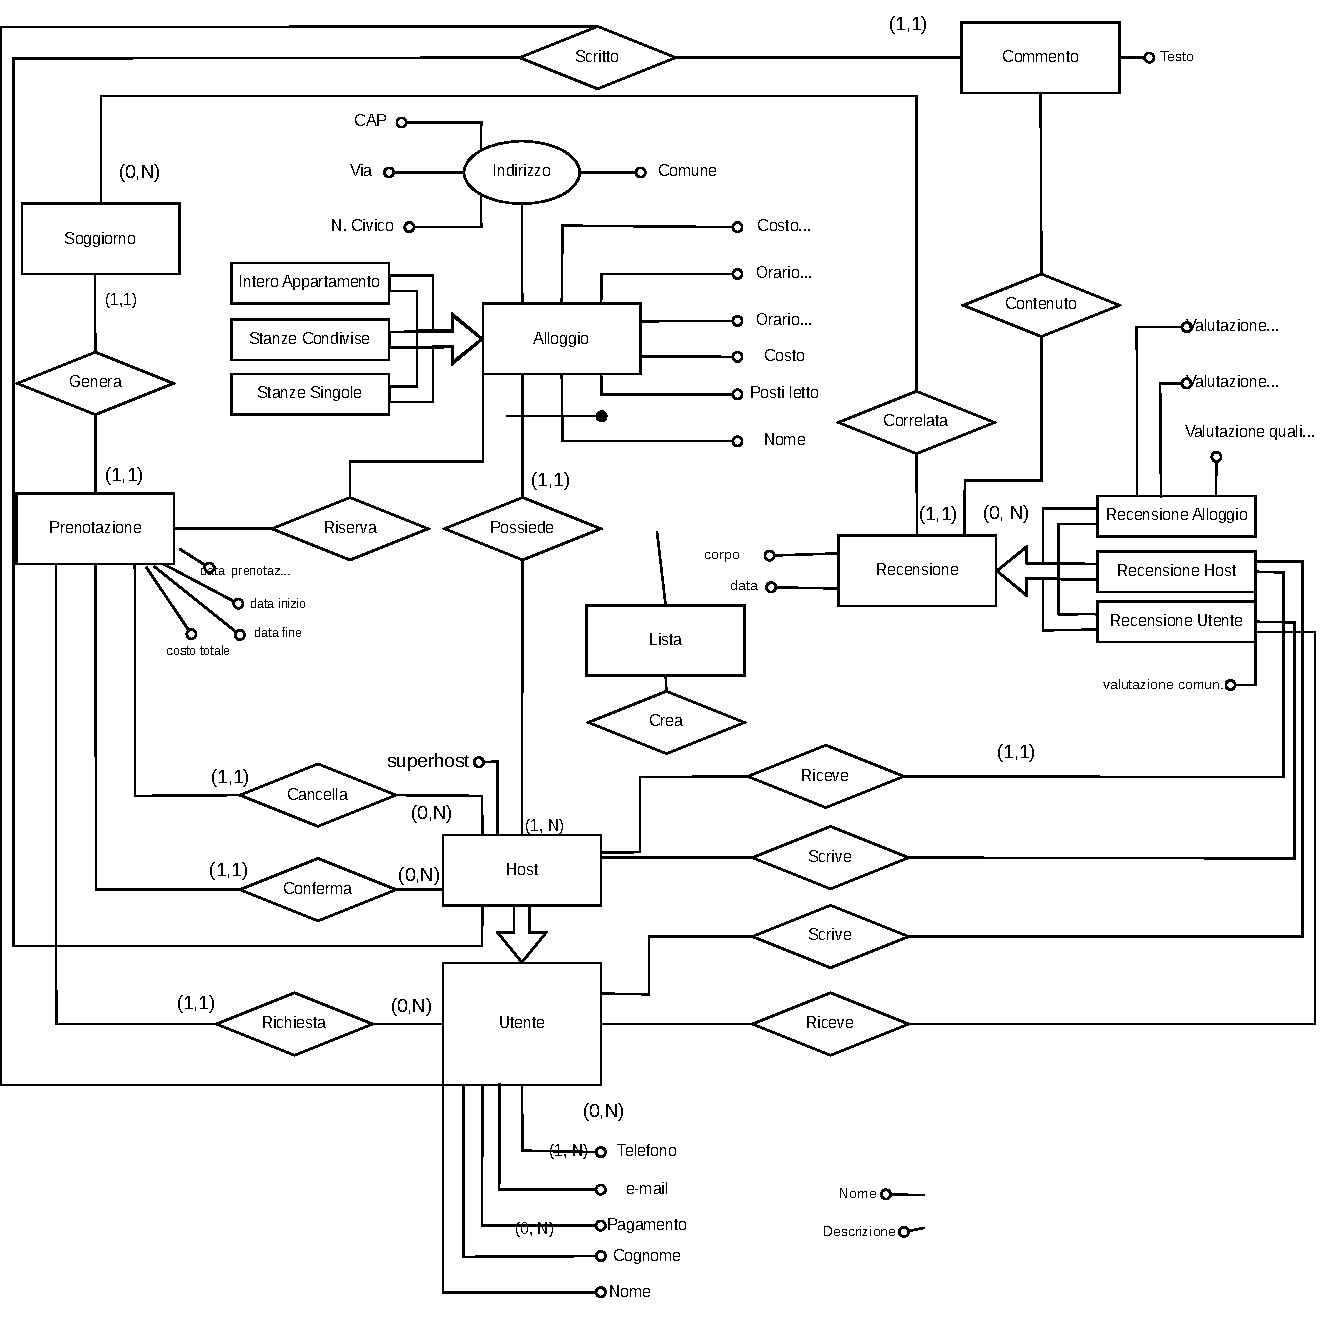
\includegraphics[width=\textwidth]{resources/ER.pdf}

\chapter{Progettazione Logica}
\section{Tavola dei Volumi}
\section{Tavola delle Operazioni}
\section{Ristrutturazione dello schema E-R}
\subsection{Analisi delle Ridondanze}
\subsection{Eliminazione delle Generalizzazioni}
\subsection{Partizionamento/Accorpamento di entità e associazioni}
\subsection{Eeventuale scelta degli identificatori principali}
\section{Schema E-R ristrutturato + Business Rules}
\section{Schema Relazionale}

\chapter{Implementazione}
\section{DDL di Creazione dei Database}
\section{DML di Popolamento di Tutte le Tabelle del Database}
\section{Qualche Operazione di cancellazione e modifica}

\end{document}